\documentclass[10pt]{article}
\usepackage{fontspec}
\usepackage{amsmath,amssymb}
\usepackage{graphicx}
\usepackage{xcolor}
\usepackage{tcolorbox}
\tcbuselibrary{skins}
\usepackage{geometry}
\geometry{
    paperwidth=612.05pt,
    paperheight=720.05pt,
    top=20pt,
    headheight=14pt,
    headsep=12pt,
    bottom=28pt,
    footskip=12pt,
    left=36pt,
    right=36pt
}
\usepackage{fancyhdr}
\usepackage{tabularx}
\usepackage{multicol}
\usepackage{tikz}

\setmainfont{Times New Roman}
\setsansfont{Arial}

\definecolor{stewartcyan}{RGB}{0, 118, 186}
\definecolor{stewartred}{RGB}{218, 41, 28}
\definecolor{stewartgray}{RGB}{120, 120, 120}

\pagestyle{fancy}
\fancyhf{}
\renewcommand{\headrulewidth}{0pt}

\begin{document}
\fancyhead[L]{\small\sffamily\textbf{\color{stewartcyan}MỤC 1.2}\quad Mô hình Toán học: Danh mục các Hàm số Cơ bản}
\fancyhead[R]{\small\sffamily\textbf{35}}

\providecommand{\techicon}{\begingroup\setlength{\fboxsep}{1.2pt}\setlength{\fboxrule}{0.8pt}\textcolor{stewartblue}{\fbox{\textcolor{stewartblue}{\sffamily\bfseries\scriptsize T}}}\endgroup\enskip}

\noindent
\begin{minipage}[t]{0.48\textwidth}
\small
\noindent
đo bằng oát ($\text{W}$) và $T$ là nhiệt độ tuyệt đối đo bằng kelvin ($\text{K}$).
\begin{enumerate}[label=(\alph*), leftmargin=*, itemsep=2pt, topsep=2pt]
    \item Vẽ đồ thị hàm số $E$ cho nhiệt độ $T$ trong khoảng từ $100\text{ K}$ đến $300\text{ K}$.
    \item Sử dụng đồ thị để mô tả sự thay đổi của năng lượng $E$ khi nhiệt độ $T$ tăng lên.
\end{enumerate}

\vspace{0.25cm}
\noindent
\textbf{\color{stewartblue}27--28}\quad Đối với mỗi biểu đồ phân tán dưới đây, hãy xác định dạng hàm số mà bạn có thể chọn làm mô hình cho dữ liệu. Giải thích sự lựa chọn của bạn.

\vspace{0.2cm}
\noindent
\begin{minipage}[t]{0.06\linewidth}
\vspace{0pt}
\textbf{27.}
\end{minipage}\hfill
\begin{minipage}[t]{0.92\linewidth}
\vspace{0pt}
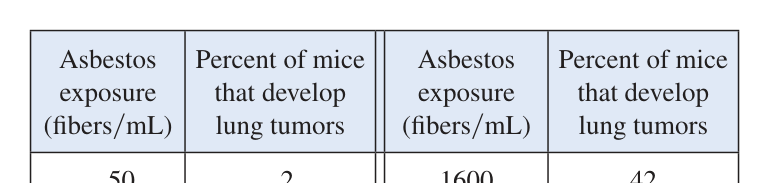
\includegraphics[width=\linewidth]{images/p0070_fig1.png}
\end{minipage}

\vspace{0.25cm}
\noindent
\begin{minipage}[t]{0.06\linewidth}
\vspace{0pt}
\textbf{28.}
\end{minipage}\hfill
\begin{minipage}[t]{0.92\linewidth}
\vspace{0pt}
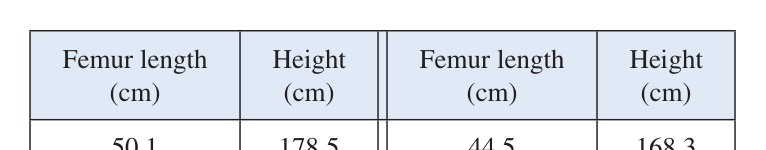
\includegraphics[width=\linewidth]{images/p0070_fig2.png}
\end{minipage}

\vspace{0.25cm}
\noindent
\techicon\textbf{29.} Bảng dưới đây cho thấy tỉ lệ mắc bệnh loét dạ dày tá tràng (suốt đời) (tính trên 100 dân số) theo các mức thu nhập hộ gia đình khác nhau được báo cáo bởi Khảo sát Phỏng vấn Y tế Quốc gia Hoa Kỳ.
\begin{enumerate}[label=(\alph*), leftmargin=*, itemsep=2pt, topsep=2pt]
    \item Hãy vẽ biểu đồ phân tán cho dữ liệu này và xác định xem mô hình tuyến tính có phù hợp hay không.
    \item Tìm và vẽ đồ thị của một mô hình tuyến tính sử dụng điểm dữ liệu đầu tiên và điểm dữ liệu cuối cùng.
    \item Tìm và vẽ đồ thị đường hồi quy tuyến tính.
    \item Sử dụng mô hình tuyến tính ở câu (c) để ước lượng tỉ lệ mắc bệnh loét cho những người có mức thu nhập \$25{,}000.
    \item Theo mô hình, khả năng một người có mức thu nhập \$80{,}000 bị loét dạ dày tá tràng là bao nhiêu?
    \item Bạn có nghĩ rằng việc áp dụng mô hình này cho một người có mức thu nhập \$200{,}000 là hợp lý không?
\end{enumerate}

\vspace{0.2cm}
\begin{center}
\renewcommand{\arraystretch}{1.12}
\begin{tabular}{|c|c|}
\hline
\rowcolor{stewarttableheader}
Thu nhập & \makecell{Tỉ lệ mắc bệnh loét\\(trên 100 dân số)} \\
\hline
\$4{,}000  & 14.1 \\
\$6{,}000  & 13.0 \\
\$8{,}000  & 13.4 \\
\$12{,}000 & 12.5 \\
\$16{,}000 & 12.0 \\
\$20{,}000 & 12.4 \\
\$30{,}000 & 10.5 \\
\$45{,}000 & 9.4 \\
\$60{,}000 & 8.2 \\
\hline
\end{tabular}
\end{center}
\end{minipage}%
\hfill
\begin{minipage}[t]{0.48\textwidth}
\small
\noindent
\techicon\textbf{30.} Khi chuột bạch trong phòng thí nghiệm tiếp xúc với các sợi amiăng, một số con đã phát triển khối u ở phổi. Bảng sau liệt kê kết quả của một số thí nghiệm do các nhà khoa học khác nhau thực hiện.
\begin{enumerate}[label=(\alph*), leftmargin=*, itemsep=2pt, topsep=2pt]
    \item Tìm phương trình đường hồi quy cho tập dữ liệu.
    \item Vẽ biểu đồ phân tán và đồ thị đường hồi quy. Đường hồi quy này có vẻ là một mô hình phù hợp cho dữ liệu không?
    \item Giao điểm với trục tung ($y$-intercept) của đường hồi quy biểu diễn điều gì?
\end{enumerate}

\vspace{0.2cm}
\begin{center}
\renewcommand{\arraystretch}{1.1}
\setlength{\tabcolsep}{3pt}
\begin{tabular}{|c|c|c|c|}
\hline
\rowcolor{stewarttableheader}
\makecell{Mức tiếp xúc\\amiăng\\(sợi/mL)} & \makecell{Tỉ lệ phần trăm\\chuột phát triển\\khối u phổi} & \makecell{Mức tiếp xúc\\amiăng\\(sợi/mL)} & \makecell{Tỉ lệ phần trăm\\chuột phát triển\\khối u phổi} \\
\hline
50   & 2  & 1600 & 42 \\
400  & 6  & 1800 & 37 \\
500  & 5  & 2000 & 38 \\
900  & 10 & 3000 & 50 \\
1100 & 26 &      &    \\
\hline
\end{tabular}
\end{center}

\vspace{0.25cm}
\noindent
\techicon\textbf{31.} Các nhà nhân chủng học sử dụng một mô hình tuyến tính liên hệ chiều dài xương đùi của con người với chiều cao. Mô hình này cho phép nhà nhân chủng học xác định chiều cao của một cá nhân khi chỉ tìm thấy một phần bộ xương (bao gồm xương đùi). Ở đây, chúng ta tìm mô hình bằng cách phân tích dữ liệu về chiều dài xương đùi và chiều cao của tám người nam giới cho trong bảng.
\begin{enumerate}[label=(\alph*), leftmargin=*, itemsep=2pt, topsep=2pt]
    \item Vẽ biểu đồ phân tán của dữ liệu.
    \item Tìm và vẽ đồ thị đường hồi quy mô hình hóa dữ liệu.
    \item Một nhà nhân chủng học tìm thấy xương đùi của người có chiều dài 53~cm. Người đó cao bao nhiêu?
\end{enumerate}

\vspace{0.2cm}
\begin{center}
\renewcommand{\arraystretch}{1.1}
\setlength{\tabcolsep}{4pt}
\begin{tabular}{|c|c|c|c|}
\hline
\rowcolor{stewarttableheader}
\makecell{Chiều dài\\xương đùi (cm)} & \makecell{Chiều cao\\(cm)} & \makecell{Chiều dài\\xương đùi (cm)} & \makecell{Chiều cao\\(cm)} \\
\hline
50.1 & 178.5 & 44.5 & 168.3 \\
48.3 & 173.6 & 42.7 & 165.0 \\
45.2 & 164.8 & 39.5 & 155.4 \\
44.7 & 163.7 & 38.0 & 155.8 \\
\hline
\end{tabular}
\end{center}

\vspace{0.25cm}
\noindent
\techicon\textbf{32.} Bảng sau cho thấy giá bán lẻ điện sinh hoạt trung bình tại Hoa Kỳ từ năm 2000 đến 2016, được tính bằng xu trên mỗi kilowatt-giờ (cents/kWh).
\begin{enumerate}[label=(\alph*), leftmargin=*, itemsep=2pt, topsep=2pt]
    \item Vẽ biểu đồ phân tán. Mô hình tuyến tính có phù hợp không?
    \item Tìm và vẽ đồ thị đường hồi quy tuyến tính.
    \item Sử dụng mô hình tuyến tính ở câu (b) để ước lượng giá bán lẻ điện trung bình trong các năm 2005 và 2017.
\end{enumerate}

\vspace{0.2cm}
\begin{center}
\renewcommand{\arraystretch}{1.1}
\setlength{\tabcolsep}{4pt}
\begin{tabular}{|c|c|c|c|}
\hline
\rowcolor{stewarttableheader}
Số năm kể từ 2000 & Xu/kWh & Số năm kể từ 2000 & Xu/kWh \\
\hline
0 & 8.24  & 10 & 11.54 \\
2 & 8.44  & 12 & 11.88 \\
4 & 8.95  & 14 & 12.52 \\
6 & 10.40 & 16 & 12.90 \\
8 & 11.26 &    &       \\
\hline
\end{tabular}

\vspace{1.5mm}
{\footnotesize\textit{Nguồn:} Cơ quan Thông tin Năng lượng Hoa Kỳ (US Energy Information Administration)}
\end{center}
\end{minipage}
\end{document}
